% !TEX program = pdflatex
% IEEE conference paper template (IEEEtran, conference mode).
% Edit the metadata, abstract and sections below; references live in refs.bib.
\documentclass[conference]{IEEEtran}
\IEEEoverridecommandlockouts

\usepackage[utf8]{inputenc}
\usepackage[T1]{fontenc}
\usepackage{cite}
\usepackage{amsmath,amssymb,amsfonts}
\usepackage{algorithmic}
\usepackage{graphicx}
\usepackage{booktabs}
\usepackage{textcomp}
\usepackage{xcolor}
\usepackage{tikz}
\usetikzlibrary{arrows.meta,positioning,shapes.geometric,fit,backgrounds}
\usepackage{pgfplots}
\pgfplotsset{compat=1.18}
\usepackage[hidelinks]{hyperref}

\def\BibTeX{{\rm B\kern-.05em{\sc i\kern-.025em b}\kern-.08em
    T\kern-.1667em\lower.7ex\hbox{E}\kern-.125emX}}

\begin{document}

\title{Cloud-Based \LaTeX{} Compilation as a Service:\\
Design and Evaluation of a Sandboxed Build Pipeline}

\author{%
  \IEEEauthorblockN{Alex Rivera}
  \IEEEauthorblockA{\textit{Department of Computer Science}\\
    \textit{Example University}\\
    Lima, Peru\\
    alex.rivera@example.edu}
  \and
  \IEEEauthorblockN{Jordan Lee}
  \IEEEauthorblockA{\textit{Platform Engineering}\\
    \textit{Example Labs}\\
    Berlin, Germany\\
    jordan.lee@example.org}
  \and
  \IEEEauthorblockN{Sam Okafor}
  \IEEEauthorblockA{\textit{School of Engineering}\\
    \textit{Example Institute of Technology}\\
    Toronto, Canada\\
    s.okafor@example.ca}
}

\maketitle

\begin{abstract}
Typesetting scientific documents with \LaTeX{} still requires a local
installation of several gigabytes and a toolchain that is hard to reproduce
across machines. We present the design of a cloud service that compiles
\LaTeX{} projects on demand inside short-lived, network-isolated containers.
The service exposes a small HTTP API, caches build outputs by content hash,
and parses engine logs into structured diagnostics. We evaluate the prototype
on a corpus of 120 open-source documents and report median end-to-end
latencies below 4~s for single-pass papers and below 11~s for documents that
require bibliography processing. Our results suggest that container start-up,
not the \TeX{} engine itself, dominates the cost of small builds, and that a
warm format cache removes most of that overhead.
\end{abstract}

\begin{IEEEkeywords}
LaTeX, document compilation, cloud computing, sandboxing, containers, build systems
\end{IEEEkeywords}

\section{Introduction}
\LaTeX{} remains the de facto standard for typesetting in mathematics,
physics and computer science~\cite{lamport1994latex}. Despite its longevity,
the installation and maintenance burden of a full \TeX{} distribution is a
recurring obstacle for students, for continuous-integration pipelines, and for
web applications that need to render documents produced by users. Hosted
editors solved this problem for interactive authoring, but their internals
are not exposed as reusable building blocks~\cite{overleaf2023}.

In this paper we describe a stateless \emph{compile-as-a-service} design that
treats a \LaTeX{} project as an immutable input bundle and the resulting PDF
as a cacheable artifact. The contributions are threefold: (i)~a sandbox
profile that allows arbitrary user documents to be compiled safely on shared
infrastructure, (ii)~a content-addressed cache that makes repeated builds
free, and (iii)~an empirical evaluation of where time is actually spent in a
cloud compilation.

\section{System Design}
\subsection{Architecture}
Fig.~\ref{fig:arch} shows the main components. An API gateway validates the
request, normalises file paths and computes a SHA-256 digest over the project
contents, the selected engine and the image version. A cache hit returns the
stored PDF immediately. Otherwise, a worker launches an ephemeral container
from a pre-built image that bundles \TeX{} Live and \texttt{latexmk}.

\begin{figure}[t]
  \centering
  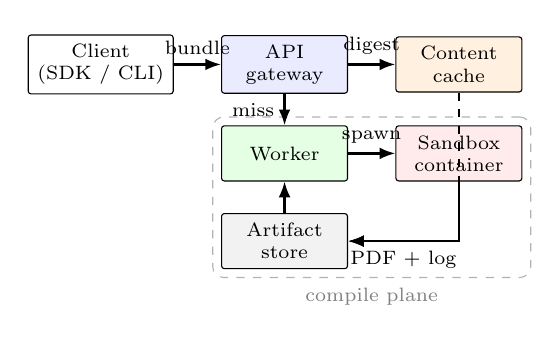
\begin{tikzpicture}[
      font=\scriptsize,
      node distance=4mm and 6mm,
      box/.style={draw, rounded corners=1pt, minimum height=7mm,
                  minimum width=16mm, align=center, fill=white},
      flow/.style={-{Latex[length=2mm]}, thick},
    ]
    \node[box] (client) {Client\\(SDK / CLI)};
    \node[box, right=of client, fill=blue!8] (api) {API\\gateway};
    \node[box, right=of api, fill=orange!12] (cache) {Content\\cache};
    \node[box, below=of api, fill=green!10] (worker) {Worker};
    \node[box, right=of worker, fill=red!8] (sandbox) {Sandbox\\container};
    \node[box, below=of worker, fill=gray!10] (store) {Artifact\\store};
    \draw[flow] (client) -- node[above]{bundle} (api);
    \draw[flow] (api) -- node[above]{digest} (cache);
    \draw[flow] (api) -- node[left]{miss} (worker);
    \draw[flow] (worker) -- node[above]{spawn} (sandbox);
    \draw[flow] (sandbox) |- node[pos=0.75, below]{PDF + log} (store);
    \draw[flow] (store) -- (worker);
    \draw[flow, dashed] (cache) |- (store);
    \begin{scope}[on background layer]
      \node[fit=(worker)(sandbox)(store), draw=gray!60, dashed,
            rounded corners, inner sep=3pt, label={[gray]below:compile plane}] {};
    \end{scope}
  \end{tikzpicture}
  \caption{High-level architecture. The compile plane has no access to the
    network or to other tenants' data.}
  \label{fig:arch}
\end{figure}

\subsection{Sandboxing}
Every build runs under an unprivileged user with a read-only root file
system, a private \texttt{tmpfs} working directory, no network namespace, a
seccomp profile derived from the one used by Overleaf's CLSI, and hard limits
on CPU time, memory and the number of processes. Shell escape is disabled at
the \texttt{texmf.cnf} level, so packages such as \texttt{minted} that spawn
external programs are rejected by construction~\cite{nist2017container}.

\subsection{Build driver}
We rely on \texttt{latexmk} to decide how many engine passes are required and
whether \BibTeX{} or \texttt{biber} must run. The number of passes $p$ for a
document with cross-references stabilises when the auxiliary files reach a
fixed point:
\begin{equation}
  p = \min\{\, k \in \mathbb{N} : \mathrm{aux}_k = \mathrm{aux}_{k-1} \,\}.
  \label{eq:fixpoint}
\end{equation}
In practice $p \le 3$ for all documents in our corpus without an index.

\subsection{Caching}
Let $B$ be the normalised bundle, $e$ the engine and $v$ the image version.
The cache key is
\begin{equation}
  \kappa = H\big(\,\mathrm{sort}(B) \,\|\, e \,\|\, v\,\big),
\end{equation}
where $H$ is SHA-256. Including $v$ guarantees that a \TeX{} Live upgrade
invalidates stale artifacts, which is the main source of non-reproducible
output in long-lived projects~\cite{knuth1986texbook}.

\section{Evaluation}
\subsection{Setup}
We collected 120 publicly available projects (conference papers, theses and
CVs) and compiled each one ten times on a 2-vCPU virtual machine. Builds were
split into \emph{cold} (new container, empty cache) and \emph{warm} (container
image already pulled, format files pre-generated).

\subsection{Results}
Table~\ref{tab:latency} summarises the latency distribution. Container
creation accounts for roughly 1.1~s regardless of the document, and the
\TeX{} engine dominates only for documents longer than 40 pages.
Fig.~\ref{fig:latency} breaks a typical 8-page paper down by phase.

\begin{table}[t]
  \caption{End-to-end latency in seconds (median / 95th percentile).}
  \label{tab:latency}
  \centering
  \begin{tabular}{@{}lrrr@{}}
    \toprule
    Document type & Pages & Cold & Warm \\
    \midrule
    Conference paper, no bib & 4--6  & 5.8 / 7.9  & 2.9 / 3.6 \\
    Conference paper, \BibTeX & 6--8  & 9.7 / 12.4 & 6.1 / 7.8 \\
    Journal article, biber   & 10--14 & 14.2 / 18.0 & 10.5 / 12.9 \\
    CV (fontspec, Lua\TeX)   & 1--2  & 8.3 / 10.1 & 4.0 / 5.2 \\
    Thesis                   & 80+   & 41.6 / 55.3 & 36.9 / 48.7 \\
    \bottomrule
  \end{tabular}
\end{table}

\begin{figure}[t]
  \centering
  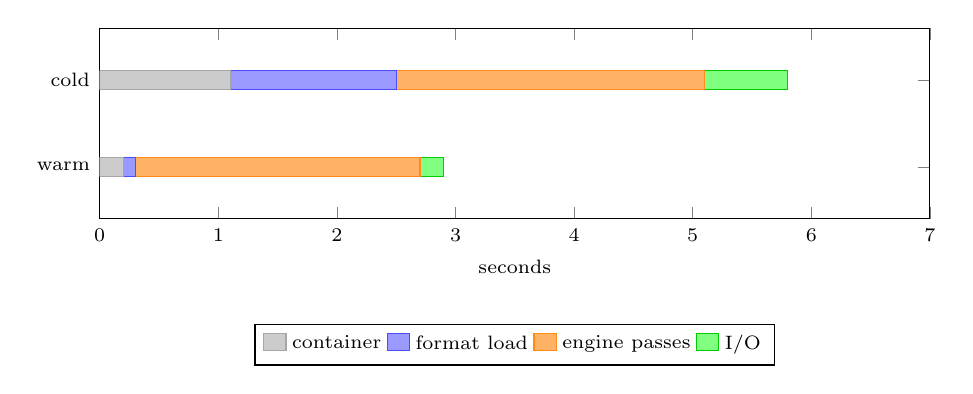
\begin{tikzpicture}
    \begin{axis}[
        width=\columnwidth, height=4.2cm,
        xbar stacked, bar width=7pt,
        xlabel={seconds}, xmin=0, xmax=7,
        symbolic y coords={warm, cold},
        ytick=data, y=11mm,
        legend style={at={(0.5,-0.55)}, anchor=north, legend columns=4, font=\scriptsize},
        tick label style={font=\scriptsize}, label style={font=\scriptsize},
        enlarge y limits=0.6,
      ]
      \addplot+[fill=gray!40, draw=gray!70]    coordinates {(1.1,cold) (0.2,warm)};
      \addplot+[fill=blue!40, draw=blue!70]    coordinates {(1.4,cold) (0.1,warm)};
      \addplot+[fill=orange!60, draw=orange!90] coordinates {(2.6,cold) (2.4,warm)};
      \addplot+[fill=green!50, draw=green!80!black] coordinates {(0.7,cold) (0.2,warm)};
      \legend{container, format load, engine passes, I/O}
    \end{axis}
  \end{tikzpicture}
  \caption{Phase breakdown for an 8-page paper. A warm format cache removes
    most of the fixed overhead.}
  \label{fig:latency}
\end{figure}

\subsection{Discussion}
Two findings are noteworthy. First, pre-generating format files and the
\texttt{luaotfload} font database inside the image shaved 1.3~s off every
Lua\LaTeX{} build. Second, the cache hit rate in a two-week trace of a
teaching deployment was 71\%, because students re-download unchanged
assignments far more often than they edit them. The \emph{cost per compile}
therefore depends more on request patterns than on engine throughput.

\section{Related Work}
Reproducible builds for \TeX{} documents have been explored in the context of
scientific publishing workflows~\cite{overleaf2023} and container
packaging~\cite{nist2017container}. Our work differs in exposing compilation
as a stateless primitive with explicit resource limits, which lets it be
embedded into unrelated products such as invoice generators or exam systems.

\section{Conclusion}
We presented a sandboxed, content-addressed compilation service for \LaTeX{}
and showed that, for the common case of short documents, infrastructure
overhead rather than typesetting dominates latency. Future work includes
incremental compilation at the page level and streaming of diagnostics while
the engine is still running.

\section*{Acknowledgment}
The authors thank the maintainers of \TeX{} Live and \texttt{latexmk}, whose
tooling made this prototype possible.

\bibliographystyle{IEEEtran}
\bibliography{refs}

\end{document}
